\documentclass[12pt,border=6pt]{standalone}
\usepackage{fontspec}
\setmainfont{BeVietnamPro}[Path=D:/IOT_Tools/downloads/fonts/,Extension=.ttf,UprightFont=*-Regular,BoldFont=*-Bold]
\usepackage{amsmath}
\usepackage{unicode-math}\setmathfont{Cambria Math}
\usepackage{xcolor}
\usepackage{tikz}
\usetikzlibrary{positioning,arrows.meta,shapes.geometric,shapes.misc,calc,fit,backgrounds,decorations.pathreplacing,shadows,3d,perspective}
\usepackage{tikz-3dplot}
\usepackage{pgfplots}\pgfplotsset{compat=1.18}
\usepgfplotslibrary{groupplots,fillbetween}
\definecolor{cDo}{HTML}{BB2025}\definecolor{cDoD}{HTML}{8E1418}\definecolor{cDoT}{HTML}{FCEBEC}
\definecolor{cXanh}{HTML}{326CE5}\definecolor{cXanhT}{HTML}{EAF0FC}
\definecolor{cLuc}{HTML}{15803D}\definecolor{cLucT}{HTML}{E6F4EA}
\definecolor{cVang}{HTML}{B45309}\definecolor{cVangT}{HTML}{FDF2E1}
\definecolor{cNavy}{HTML}{1E293B}\definecolor{cMuc}{HTML}{1F2937}\definecolor{cXam}{HTML}{4B5563}
\definecolor{cXamT}{HTML}{F3F4F6}\definecolor{cVien}{HTML}{DDE1E6}\definecolor{cTim}{HTML}{6D28D9}\definecolor{cTimT}{HTML}{F1EBFD}
\pgfplotsset{slide/.style={tick label style={font=\small}, label style={font=\small}, scaled ticks=false,
  /pgf/number format/fixed, /pgf/number format/use comma, /pgf/number format/1000 sep={\,},
  legend style={font=\small,draw=none,fill=none}, axis line style={cXam}, major tick style={cXam},
  grid style={cVien}}}
\pgfkeys{/pgf/number format/assume math mode=true}
\begin{document}
% F01 · S01, S35 · drone Quad X nhìn chéo 3/4 từ trên: 4 cần, 4 motor + đĩa cánh, stack giữa, cột GPS ở đuôi,
% TFmini ở mũi (tia đỏ), camera mép trước chúc ~30°, ESP32 bên hông, sóng Wi-Fi tới laptop.
% Nguồn hình dạng: facts/01-phan-cung.md mục 1, 6; chiều quay mục 2 (trước-phải + sau-trái CCW, trước-trái + sau-phải CW).
% Khung slide 8,1 x 6,8 in. Toạ độ drone: x = mũi, y = trái, z = lên; R = 5 (tâm tới motor), cả drone phóng 1,2.
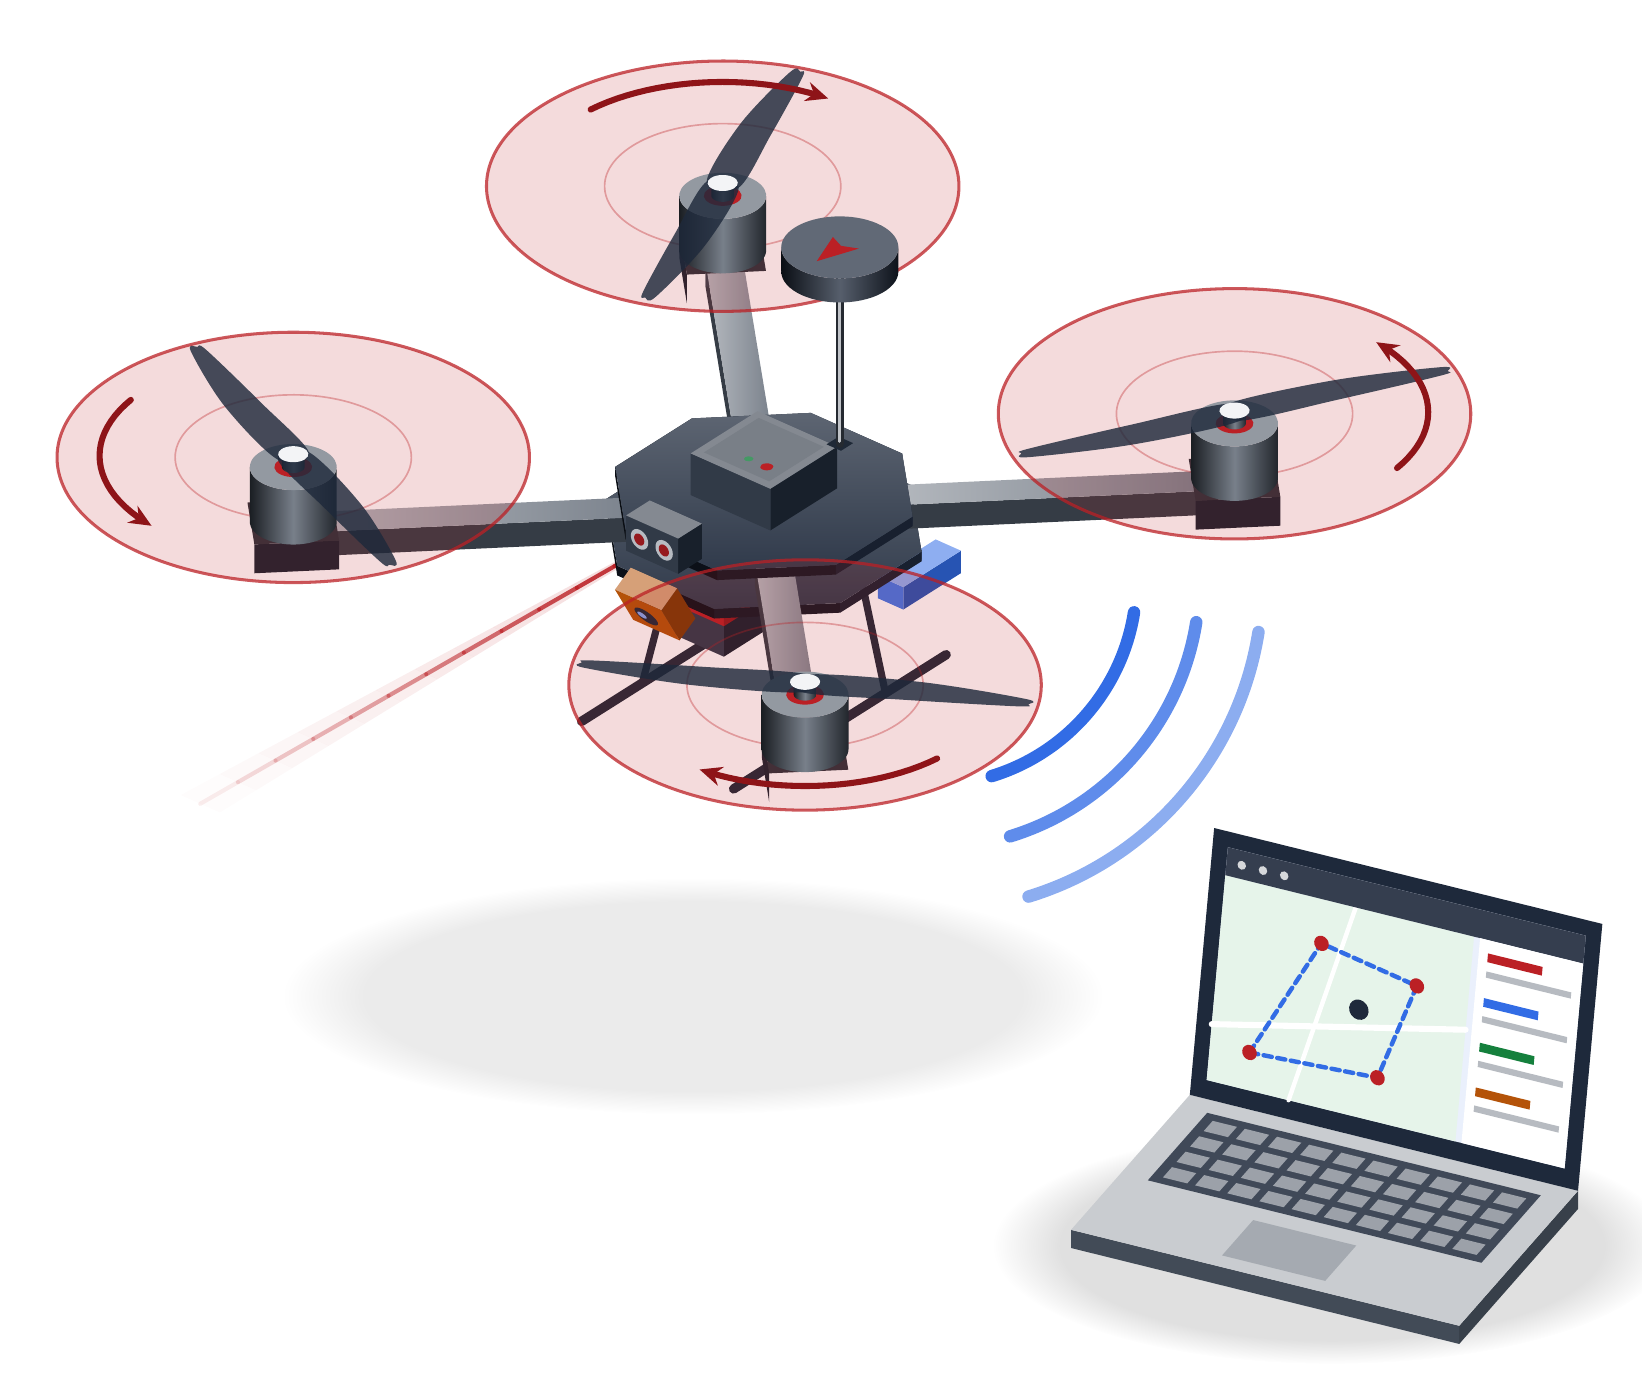
\begin{tikzpicture}[line join=round,line cap=round]
\tdplotsetmaincoords{58}{130}
\useasboundingbox (-9.35,-10.55) rectangle (10.80,6.30);
% ---------- hộp trục thẳng: chỉ 3 mặt thấy được (+z, +x, +y) với góc nhìn này
\newcommand\bx[7]{%
  \fill[#7!78!black] (#1,#4,#5) -- (#2,#4,#5) -- (#2,#4,#6) -- (#1,#4,#6) -- cycle;
  \fill[#7!92!white] (#2,#3,#5) -- (#2,#4,#5) -- (#2,#4,#6) -- (#2,#3,#6) -- cycle;
  \fill[#7!55!white] (#1,#3,#6) -- (#2,#3,#6) -- (#2,#4,#6) -- (#1,#4,#6) -- cycle;}
% ---------- trụ đứng: \cyl{x}{y}{z0}{z1}{r}{màu thân}{màu nắp}
\newcommand\cyl[7]{%
  \shade[left color=#6!35!black,right color=#6!45!black,middle color=#6!75!white]
    plot[domain=130:-50,samples=30,variable=\t] ({#1+#5*cos(\t)},{#2+#5*sin(\t)},#3)
    -- plot[domain=-50:130,samples=30,variable=\t] ({#1+#5*cos(\t)},{#2+#5*sin(\t)},#4) -- cycle;
  \fill[#7] (#1,#2,#4) circle (#5);}
% ---------- lăng trụ bát giác (tấm khung): \oct{z0}{z1}{bán kính}{màu}
\newcommand\oct[4]{%
  \foreach \k in {0,...,7}{
    \pgfmathsetmacro\aa{22.5+45*\k}\pgfmathsetmacro\ab{67.5+45*\k}
    \pgfmathsetmacro\lt{int(62+28*cos(45*\k+45-140))}
    \fill[#4!\lt!black] ({#3*cos(\aa)},{#3*sin(\aa)},#1) -- ({#3*cos(\ab)},{#3*sin(\ab)},#1)
      -- ({#3*cos(\ab)},{#3*sin(\ab)},#2) -- ({#3*cos(\aa)},{#3*sin(\aa)},#2) -- cycle;}
  \shade[top color=#4!72!white,bottom color=#4!92!white]
    ({#3*cos(22.5)},{#3*sin(22.5)},#2) \foreach \k in {1,...,7}{-- ({#3*cos(22.5+45*\k)},{#3*sin(22.5+45*\k)},#2)} -- cycle;}
% ---------- cần: \arm{góc}{dấu mặt bên thấy được}
\newcommand\arm[2]{%
  \tdplotsetrotatedcoords{#1}{0}{0}
  \begin{scope}[tdplot_rotated_coords]
    \fill[cXam!70!black] (1.2,{#2*0.2},-0.02) -- (4.8,{#2*0.2},-0.02) -- (4.8,{#2*0.2},0.28) -- (1.2,{#2*0.2},0.28) -- cycle;
    \fill[cXam!80!black] (4.8,-0.2,-0.02) -- (4.8,0.2,-0.02) -- (4.8,0.2,0.28) -- (4.8,-0.2,0.28) -- cycle;
    \shade[left color=cXam!40!white,right color=cXam!75!white]
      (1.2,-0.2,0.28) -- (4.8,-0.2,0.28) -- (4.8,0.2,0.28) -- (1.2,0.2,0.28) -- cycle;
    % đế motor
    \fill[cMuc!85!black] (4.55,{#2*0.42},-0.06) -- (5.45,{#2*0.42},-0.06) -- (5.45,{#2*0.42},0.30) -- (4.55,{#2*0.42},0.30) -- cycle;
    \fill[cXam!60!black] (4.55,-0.42,0.30) -- (5.45,-0.42,0.30) -- (5.45,0.42,0.30) -- (4.55,0.42,0.30) -- cycle;
  \end{scope}}
% ---------- motor + cánh: \prop{góc cần}{góc cánh}{1 = CCW, -1 = CW}
\newcommand\prop[3]{%
  \pgfmathsetmacro\mx{5*cos(#1)}\pgfmathsetmacro\my{5*sin(#1)}
  % đĩa cánh (vẽ trước để motor giữ màu xám)
  \fill[cDo,opacity=.16] (\mx,\my,1.10) circle (2.5);
  \draw[cDo,opacity=.75,line width=1.1pt] (\mx,\my,1.10) circle (2.5);
  \draw[cDo,opacity=.35,line width=0.6pt] (\mx,\my,1.10) circle (1.25);
  \cyl{\mx}{\my}{0.30}{0.98}{0.46}{cXam}{cXam!60!white}
  \fill[cDo] (\mx,\my,0.98) circle (0.20);
  \cyl{\mx}{\my}{0.98}{1.12}{0.12}{cXam}{cXamT}

  % 2 lá cánh
  \foreach \s in {0,180}{
    \pgfmathsetmacro\b{#2+\s}
    \fill[cNavy,opacity=.82] plot[smooth cycle,tension=.55] coordinates {
      ({\mx+0.18*cos(\b+90)},{\my+0.18*sin(\b+90)},1.12)
      ({\mx+1.2*cos(\b)+0.24*cos(\b+90)},{\my+1.2*sin(\b)+0.24*sin(\b+90)},1.12)
      ({\mx+2.35*cos(\b)+0.10*cos(\b+90)},{\my+2.35*sin(\b)+0.10*sin(\b+90)},1.12)
      ({\mx+2.4*cos(\b)},{\my+2.4*sin(\b)},1.12)
      ({\mx+2.3*cos(\b)-0.06*cos(\b+90)},{\my+2.3*sin(\b)-0.06*sin(\b+90)},1.12)
      ({\mx+1.1*cos(\b)-0.14*cos(\b+90)},{\my+1.1*sin(\b)-0.14*sin(\b+90)},1.12)
      ({\mx-0.18*cos(\b+90)},{\my-0.18*sin(\b+90)},1.12)};}
  \fill[cXamT] (\mx,\my,1.14) circle (0.16);
  % mũi tên chiều quay
  \pgfmathsetmacro\sa{#1-#3*38}\pgfmathsetmacro\sb{#1+#3*38}
  \draw[cDoD,line width=2.2pt,-{Stealth[length=8pt,width=7pt]}]
    plot[domain=\sa:\sb,samples=24,variable=\t] ({\mx+2.05*cos(\t)},{\my+2.05*sin(\t)},1.12);}
\newcommand\qd[4]{(#1,#2) -- (#3,#2) -- (#3,#4) -- (#1,#4) -- cycle}
% bóng mềm dưới drone (vẽ đầu tiên)
\fill[black,opacity=.08,path fading=circle with fuzzy edge 20 percent] (-0.9,-6.0) ellipse (5.2 and 1.5);
% ================= laptop (góc phải dưới), mặt trước hướng phương vị 15°
\begin{scope}[shift={(7.12,-8.95)},scale=0.85]
\begin{scope}[tdplot_main_coords]
  \pgfmathsetmacro\fx{cos(15)}\pgfmathsetmacro\fy{sin(15)}\pgfmathsetmacro\wx{-sin(15)}\pgfmathsetmacro\wy{cos(15)}
  \coordinate (BFL) at ({2.1*\fx-3.2*\wx},{2.1*\fy-3.2*\wy},0);
  \coordinate (BFR) at ({2.1*\fx+3.2*\wx},{2.1*\fy+3.2*\wy},0);
  \coordinate (BBR) at ({-2.1*\fx+3.2*\wx},{-2.1*\fy+3.2*\wy},0);
  \coordinate (BBL) at ({-2.1*\fx-3.2*\wx},{-2.1*\fy-3.2*\wy},0);
  \coordinate (TFL) at ({2.1*\fx-3.2*\wx},{2.1*\fy-3.2*\wy},0.32);
  \coordinate (TFR) at ({2.1*\fx+3.2*\wx},{2.1*\fy+3.2*\wy},0.32);
  \coordinate (TBR) at ({-2.1*\fx+3.2*\wx},{-2.1*\fy+3.2*\wy},0.32);
  \coordinate (TBL) at ({-2.1*\fx-3.2*\wx},{-2.1*\fy-3.2*\wy},0.32);
  \coordinate (Lsh) at (0.3,0.4,0);
  \coordinate (Uw) at ({\wx},{\wy},0);
  \coordinate (Uf) at ({-\fx},{-\fy},0);
  \coordinate (Uu) at ({-0.2*\fx},{-0.2*\fy},0.98);
  \coordinate (O) at (0,0,0);
\end{scope}
\end{scope}
% bóng mềm dưới laptop
\fill[black,opacity=.12,path fading=circle with fuzzy edge 20 percent] (Lsh) ellipse (4.3 and 1.5);
% mặt bên phải + mặt trước của đế
\fill[cXam!75!black] (BFR) -- (BBR) -- (TBR) -- (TFR) -- cycle;
\fill[cXam!88!black] (BFL) -- (BFR) -- (TFR) -- (TFL) -- cycle;
\fill[cXam!30!white] (TFL) -- (TFR) -- (TBR) -- (TBL) -- cycle;
% bàn phím + touchpad trên mặt đế (mặt phẳng w, -f)
\begin{scope}[shift={(TFL)},x={($(Uw)-(O)$)},y={($(Uf)-(O)$)}]
  \fill[cNavy!85!white] \qd{0.45}{1.75}{5.95}{3.85};
  \foreach \r in {0,...,3}\foreach \c in {0,...,9}
    \fill[cXam!55!white] \qd{0.62+0.53*\c}{1.92+0.48*\r}{1.02+0.53*\c}{2.24+0.48*\r};
  \fill[cXam!50!white] \qd{2.35}{0.30}{4.05}{1.40};
\end{scope}
% màn hình (bản lề ở mép sau, ngả 12°)
\begin{scope}[shift={(TBL)},x={($(Uw)-(O)$)},y={($(Uu)-(O)$)}]
  \fill[cNavy] \qd{0}{0}{6.4}{4.3};
  \fill[cXanhT] \qd{0.25}{0.30}{6.15}{4.05};
  % bản đồ nhỏ của web GCS
  \fill[cLucT] \qd{0.25}{0.30}{4.35}{3.60};
  \draw[white,line width=2.2pt] (0.25,1.2) -- (4.35,2.1);
  \draw[white,line width=1.6pt] (1.6,0.30) -- (2.4,3.60);
  \draw[cXanh,line width=1.6pt,dash pattern=on 3pt off 2pt] (0.9,0.9) -- (1.9,2.9) -- (3.5,2.6) -- (3.0,1.0) -- cycle;
  \foreach \p in {(0.9,0.9),(1.9,2.9),(3.5,2.6),(3.0,1.0)} \fill[cDo] \p circle (0.12);
  \fill[cNavy] (2.6,2.0) circle (0.16);
  \fill[cNavy!90!white] \qd{0.25}{3.60}{6.15}{4.05};
  \foreach \i in {0,1,2} \fill[white,opacity=.8] ({0.5+0.35*\i},3.82) circle (0.07);
  % cột số liệu
  \fill[white] \qd{4.45}{0.30}{6.15}{3.60};
  \foreach \i/\c in {0/cDo,1/cXanh,2/cLuc,3/cVang}{
    \fill[\c] \qd{4.6}{3.25-0.72*\i}{5.5}{3.39-0.72*\i};
    \fill[cXam!40!white] \qd{4.6}{3.0-0.72*\i}{6.0}{3.1-0.72*\i};}
\end{scope}
% ================= drone
\begin{scope}[scale=1.2]

\begin{scope}[tdplot_main_coords]
  % --- tia TFmini (vẽ trước, mảnh, mờ dần)
  \foreach \i in {0,...,11}{
    \pgfmathsetmacro\ta{1.84+0.62*\i}\pgfmathsetmacro\tb{\ta+0.62}\pgfmathsetmacro\op{0.95*(1-\i/12)}
    \pgfmathsetmacro\opf{0.16*(1-\i/12)}
    \fill[cDo,opacity=\opf] (\ta,{-0.04-0.031*(\ta-1.84)},{0.62+0.044*(\ta-1.84)})
      -- (\tb,{-0.04-0.031*(\tb-1.84)},{0.62+0.044*(\tb-1.84)}) -- (\tb,{0.04+0.031*(\tb-1.84)},{0.62+0.044*(\tb-1.84)})
      -- (\ta,{0.04+0.031*(\ta-1.84)},{0.62+0.044*(\ta-1.84)}) -- cycle;
    \draw[cDo,opacity=\op,line width=1.5pt] (\ta,0,{0.62+0.044*(\ta-1.84)}) -- (\tb,0,{0.62+0.044*(\tb-1.84)});}
  % --- chân đáp phía sau (y < 0)
  \draw[cMuc,line width=2.6pt] (-0.75,-0.55,-0.12) -- (-0.75,-1.05,-2.05);
  \draw[cMuc,line width=2.6pt] (0.75,-0.55,-0.12) -- (0.75,-1.05,-2.05);
  \draw[cMuc,line width=3.4pt] (-1.75,-1.05,-2.05) -- (1.75,-1.05,-2.05);
  % --- pin dưới tấm đế
  \bx{-1.35}{1.35}{-0.58}{0.58}{-0.78}{-0.14}{cNavy}
  \fill[cDo] (1.35,-0.58,-0.40) -- (1.35,0.58,-0.40) -- (1.35,0.58,-0.30) -- (1.35,-0.58,-0.30) -- cycle;
  \fill[cDo!80!black] (-1.35,0.58,-0.40) -- (1.35,0.58,-0.40) -- (1.35,0.58,-0.30) -- (-1.35,0.58,-0.30) -- cycle;
  % --- chân đáp phía trước (y > 0)
  \draw[cMuc,line width=2.6pt] (-0.75,0.55,-0.12) -- (-0.75,1.05,-2.05);
  \draw[cMuc,line width=2.6pt] (0.75,0.55,-0.12) -- (0.75,1.05,-2.05);
  \draw[cMuc,line width=3.4pt] (-1.75,1.05,-2.05) -- (1.75,1.05,-2.05);
  % --- ESP32 DroneBridge (hông trái, tầng dưới)
  \bx{-1.10}{-0.15}{1.45}{1.80}{-0.42}{-0.14}{cXanh}
  % --- tấm đế
  \oct{-0.14}{-0.02}{1.75}{cNavy}
  % --- 4 cần (sau tới trước)
  \arm{-135}{1}
  \arm{135}{-1}
  \arm{-45}{1}
  \arm{45}{-1}
  % --- camera ESP32-S3 + OV3660 ở mép trước, chúc 30°
  \pgfmathsetmacro\dX{cos(30)}\pgfmathsetmacro\dZ{-sin(30)}\pgfmathsetmacro\uX{sin(30)}\pgfmathsetmacro\uZ{cos(30)}
  \coordinate (cam) at (1.92,0,-0.22);
  \fill[cVang!70!black] ($(cam)+(-0.30*\dX-0.30*\uX,0.32,-0.30*\dZ-0.30*\uZ)$) -- ($(cam)+(-0.30*\uX,0.32,-0.30*\uZ)$)
    -- ($(cam)+(0.30*\uX,0.32,0.30*\uZ)$) -- ($(cam)+(-0.30*\dX+0.30*\uX,0.32,-0.30*\dZ+0.30*\uZ)$) -- cycle;
  \fill[cVang!55!white] ($(cam)+(-0.30*\dX+0.30*\uX,-0.32,-0.30*\dZ+0.30*\uZ)$) -- ($(cam)+(0.30*\uX,-0.32,0.30*\uZ)$)
    -- ($(cam)+(0.30*\uX,0.32,0.30*\uZ)$) -- ($(cam)+(-0.30*\dX+0.30*\uX,0.32,-0.30*\dZ+0.30*\uZ)$) -- cycle;
  \fill[cVang] ($(cam)+(-0.30*\uX,-0.32,-0.30*\uZ)$) -- ($(cam)+(-0.30*\uX,0.32,-0.30*\uZ)$)
    -- ($(cam)+(0.30*\uX,0.32,0.30*\uZ)$) -- ($(cam)+(0.30*\uX,-0.32,0.30*\uZ)$) -- cycle;
  \fill[cMuc] plot[domain=0:360,samples=30,variable=\t] ({1.92+0.02*\dX+0.15*sin(\t)*\uX},{0.15*cos(\t)},{-0.22+0.02*\dZ+0.15*sin(\t)*\uZ});
  \fill[cXanh!60!white] plot[domain=0:360,samples=30,variable=\t] ({1.93+0.03*\dX+0.06*sin(\t)*\uX+0.03*\uX},{0.06*cos(\t)-0.03},{-0.22+0.03*\dZ+0.06*sin(\t)*\uZ+0.03*\uZ});
  % --- motor + cánh phía sau
  \prop{-135}{20}{-1}
  % --- tấm trên, stack, GPS, TFmini
  \oct{0.28}{0.40}{1.65}{cNavy}
  \bx{-0.55}{0.55}{-0.55}{0.55}{0.40}{0.92}{cMuc}
  \fill[cMuc!60!white] (-0.45,-0.45,0.925) -- (0.45,-0.45,0.925) -- (0.45,0.45,0.925) -- (-0.45,0.45,0.925) -- cycle;
  \fill[cDo] (0.25,0.25,0.93) circle (0.07);
  \fill[cLuc!80!white] (0.25,0.0,0.93) circle (0.05);
  % cột GPS ở đuôi
  \fill[cMuc] (-1.35,-0.10,0.40) -- (-1.15,-0.10,0.40) -- (-1.15,0.10,0.40) -- (-1.35,0.10,0.40) -- cycle;
  \draw[cXam!50!black,line width=3pt] (-1.25,0,0.40) -- (-1.25,0,2.55);
  \draw[cXam!35!white,line width=1pt] (-1.22,0.02,0.45) -- (-1.22,0.02,2.50);
  \cyl{-1.25}{0}{2.55}{2.85}{0.62}{cNavy}{cNavy!70!white}
  \fill[cDo] (-1.25+0.38,0,2.86) -- (-1.25-0.10,0.18,2.86) -- (-1.25-0.02,0,2.86) -- (-1.25-0.10,-0.18,2.86) -- cycle;
  % TFmini ở mũi
  \bx{1.45}{1.84}{-0.36}{0.36}{0.40}{0.84}{cMuc}
  \foreach \yy in {-0.17,0.17}{
    \fill[cXam!40!white] plot[domain=0:360,samples=24,variable=\t] (1.845,{\yy+0.12*cos(\t)},{0.62+0.12*sin(\t)});
    \fill[cDo!80!black] plot[domain=0:360,samples=24,variable=\t] (1.85,{\yy+0.07*cos(\t)},{0.62+0.07*sin(\t)});}
  % --- motor + cánh hai bên và phía trước
  \prop{135}{-30}{1}
  \prop{-45}{65}{1}
  \prop{45}{-60}{-1}
\end{scope}
% sóng Wi-Fi từ ESP32 tới laptop
\begin{scope}[tdplot_main_coords]\coordinate (wifi) at (-0.62,1.80,-0.28);\end{scope}
\end{scope}
\foreach \r/\o in {2.6/1,3.4/.78,4.2/.56}
  \draw[cXanh,line width=4.5pt,opacity=\o] ($(wifi)+(-73:\r)$) arc[start angle=-73,end angle=-9,radius=\r];

\end{tikzpicture}

\end{document}
